\documentclass[a4paper, 10pt, ]{article}

\usepackage[slovak]{babel}





\usepackage[utf8]{inputenc}
\usepackage[T1]{fontenc}

\usepackage[left=4cm,
			right=4cm,
            % left=2.5cm,
			% right=5.5cm,
			top=2.1cm,
			bottom=2.6cm,
			footskip=7.5mm,
			% twoside,
			marginparwidth=3.0cm,
			%showframe,
			]{geometry}

\usepackage{graphicx}
\usepackage[dvipsnames]{xcolor}
% https://en.wikibooks.org/wiki/LaTeX/Colors


% ------------------------------

\usepackage{lmodern}

\usepackage[tt={oldstyle=false,proportional=true,monowidth}]{cfr-lm}

% ------------------------------

\usepackage{amsmath}
\usepackage{amssymb}
\usepackage{amsthm}

\usepackage{booktabs}
\usepackage{multirow}
\usepackage{array}
\usepackage{dcolumn}


\usepackage[singlelinecheck=true]{subfig}


% ------------------------------


\def\naT{\mathsf{T}}

\hyphenpenalty=6000
\tolerance=1000




% ------------------------------


\makeatletter

	\def\@seccntformat#1{\protect\makebox[0pt][r]{\csname the#1\endcsname\hspace{4mm}}}

	\def\cleardoublepage{\clearpage\if@twoside \ifodd\c@page\else
	\hbox{}
	\vspace*{\fill}
	\begin{center}
	\phantom{}
	\end{center}
	\vspace{\fill}
	\thispagestyle{empty}
	\newpage
	\if@twocolumn\hbox{}\newpage\fi\fi\fi}

	\newcommand\figcaption{\def\@captype{figure}\caption}
	\newcommand\tabcaption{\def\@captype{table}\caption}

\makeatother


% ------------------------------




\usepackage{fancyhdr}
\fancypagestyle{plain}{%
\fancyhf{} % clear all header and footer fields
\fancyfoot[C]{\sffamily {\bfseries \thepage}\ | {\scriptsize\oznacenieCasti}}
\renewcommand{\headrulewidth}{0pt}
\renewcommand{\footrulewidth}{0pt}}
\pagestyle{plain}


% ------------------------------


\usepackage{titlesec}
\titleformat{\paragraph}[hang]{\sffamily  \bfseries}{}{0pt}{}
\titlespacing*{\paragraph}{0mm}{3mm}{1mm}
\titlespacing*{\subparagraph}{0mm}{3mm}{1mm}

\titleformat*{\section}{\sffamily\Large\bfseries}
\titleformat*{\subsection}{\sffamily\large\bfseries}
\titleformat*{\subsubsection}{\sffamily\normalsize\bfseries}






% ------------------------------

\PassOptionsToPackage{hyphens}{url}
\usepackage[pdfauthor={},
			pdftitle={},
			pdfsubject={},
			pdfkeywords={},
			% hidelinks,
			colorlinks=false,
			breaklinks,
			]{hyperref}


% ------------------------------


\graphicspath{%
{../fig_standalone/}%
{../../PY/fig/}%
{../../PY/jupynotex/fig/}%
{../../ML/fig/}%
{./fig/}%
}



% ------------------------------

\usepackage{enumitem}

\usepackage{lettrine}

% ------------------------------


\usepackage{microtype}


% ------------------------------

\usepackage[titles]{tocloft}

\setlength{\cftsecindent}{-12mm}
\setlength{\cftsecnumwidth}{12mm}
\renewcommand{\cftsecpresnum}{\hfill}
\renewcommand{\cftsecaftersnum}{\hspace{4mm}}

\setlength{\cftsubsecindent}{-12mm}
\setlength{\cftsubsecnumwidth}{16mm} % 12 + 4
\renewcommand{\cftsubsecpresnum}{\hfill}
\renewcommand{\cftsubsecaftersnum}{\hspace{8mm}} % 4 + 4 mm

\setlength{\cftsubsubsecindent}{-12mm}
\setlength{\cftsubsubsecnumwidth}{20mm} % 12 + 4 + 4
\renewcommand{\cftsubsubsecpresnum}{\hfill}
\renewcommand{\cftsubsubsecaftersnum}{\hspace{12mm}} % 4 + 4 + 4 mm

\renewcommand{\cftsecpagefont}{\lstyle \bfseries}
\renewcommand{\cftsubsecpagefont}{\lstyle}
\renewcommand{\cftsubsubsecpagefont}{\lstyle}



\setlength{\cftparaindent}{-16mm}
\setlength{\cftparanumwidth}{28mm} % 16 + 4 + 4 + 4
\renewcommand{\cftparapresnum}{\hfill}
\renewcommand{\cftparaaftersnum}{\hspace{16mm}} % 4 + 4 + 4 + 4 mm








% ------------------------------

\usepackage{listings}



\renewcommand{\lstlistingname}{Výpis kódu}
\renewcommand{\lstlistlistingname}{Výpisy kódu}




%New colors defined below
\definecolor{codegreen}{rgb}{0,0.6,0}
\definecolor{codegray}{rgb}{0.5,0.5,0.5}
\definecolor{codepurple}{rgb}{0.58,0,0.82}
\definecolor{backcolour}{rgb}{0.95,0.95,0.95}

%Code listing style named "mystyle"
\lstdefinestyle{mystyle}{
  backgroundcolor=\color{backcolour},
  commentstyle=\fontfamily{lmtt}\fontsize{8.5pt}{8.75pt}\selectfont\color{codegreen},
  keywordstyle=\fontfamily{lmtt}\fontsize{8.5pt}{8.75pt}\selectfont\bfseries\color{Blue},
  stringstyle=\fontfamily{lmtt}\fontsize{8.5pt}{8.75pt}\selectfont\color{codepurple},
  basicstyle=\fontfamily{lmtt}\fontsize{8.5pt}{8.75pt}\selectfont,
  breakatwhitespace=false,
  breaklines=true,
  captionpos=t,
  keepspaces=true,
  numbers=left,
  numbersep=4mm,
  numberstyle=\fontfamily{lmtt}\fontsize{8.5pt}{8.75pt}\selectfont\color{lightgray},
  showspaces=false,
  showstringspaces=false,
  showtabs=false,
  tabsize=2,
  % xleftmargin=10pt,
  framesep=10pt,
  language=Python,
  escapechar=|,
}


\lstset{
    inputencoding=utf8,
    extendedchars=true,
    literate=%
    {á}{{\'a}}1
    {č}{{\v{c}}}1
    {ď}{{\v{d}}}1
    {é}{{\'e}}1
    {ě}{{\v{e}}}1
    {í}{{\'i}}1
    {ň}{{\v{n}}}1
    {ó}{{\'o}}1
    {ř}{{\v{r}}}1
    {š}{{\v{s}}}1
    {ť}{{\v{t}}}1
    {ú}{{\'u}}1
    {ů}{{\r{u}}}1
    {ý}{{\'y}}1
    {ž}{{\v{z}}}1
    {Á}{{\'A}}1
    {Č}{{\v{C}}}1
    {Ď}{{\v{D}}}1
    {É}{{\'E}}1
    {Ě}{{\v{E}}}1
    {Í}{{\'I}}1
    {Ň}{{\v{N}}}1
    {Ó}{{\'O}}1
    {Ř}{{\v{R}}}1
    {Š}{{\v{S}}}1
    {Ť}{{\v{T}}}1
    {Ú}{{\'U}}1
    {Ů}{{\r{U}}}1
    {Ý}{{\'Y}}1
    {Ž}{{\v{Z}}}1
    {ô}{{\^{o}}}1
}


% ------------------------------


\usepackage{caption}

\DeclareCaptionFormat{odsadene}{\protect\makebox[0pt][r]{#1#2\hspace{4mm}}#3\par}
\DeclareCaptionLabelSeparator{lendvojbodka}{:}
% \DeclareCaptionFont{lightgray}{\color{lightgray}}
\DeclareCaptionFont{lightgray}{\fontfamily{lmtt}\fontsize{8.5pt}{8.75pt}\selectfont\color{lightgray}}

\captionsetup[lstlisting]{format=odsadene, labelsep=lendvojbodka, justification=raggedright, singlelinecheck=false, labelfont={sf, lightgray},}


% ------------------------------





% ------------------------------

\usepackage[backend=biber,
            style=numeric,
            sorting=none,
            ]{biblatex}
\DeclareSourcemap{
    \maps[datatype=bibtex]{
        \map{
        \step[fieldset=note, null]
        }
        \map{
        \step[fieldset=file, null]
        }        
        % \map{
        % \step[fieldset=url, null]        
        % }
        \map{
        \step[fieldset=eprint, null]
        }
    }
}


\addbibresource{E:/_CurrentContent/01_work_repo/bibLaTeXDB/bibLaTeXDB.bib} % nonpublic data





\def\oznacenieCasti{MRS03 - ZS2024}





\begin{document}


\lstset{%
style=mystyle,
rangebeginprefix=\#\#\#\ cellB\ ,%
rangebeginsuffix=\ \#\#\#,%
rangeendprefix=\#\#\#\ cellE\ ,%
rangeendsuffix=\ \#\#\#,%
includerangemarker=false,
}






\fontsize{12pt}{22pt}\selectfont

\centerline{\textsf{Modelovanie a riadenie systémov} \hfill \textsf{\oznacenieCasti}}

\fontsize{18pt}{22pt}\selectfont





\begin{flushleft}
	\textbf{\textsf{Cvičenie druhé a tretie}}
\end{flushleft}






\normalsize

\bigskip

{\hypersetup{hidelinks}

\tableofcontents

}

\bigskip

\vspace{18pt}



\noindent
\lettrine[lines=3, nindent=0pt]{C}{ieľom} cvičení sú témy týkajúce sa schematického znázornenia dynamického systému daného diferenciálnou rovnicou (alebo sústavou dif. rovníc), témy týkajúce sa rozkladu dif. rovnice vyššieho rádu na sústavu rovníc prvého rádu a~získanie numerického riešenia s využitím softvéru Simulink a MATLAB (prípadne iného).














\section{Cvičenie druhé} 




\subsection{Úloha 1} \label{cv2u1}

Majme dynamický systém daný diferenciálnou rovnicou v tvare
\begin{equation} \label{eq:DR2R}
    \ddot y(t) + a_1 \dot y(t) + a_0 y(t) = b_0 u(t) \qquad y(0) = y_0 \qquad \dot y(0) = z_0
\end{equation}
kde $a_0$, $a_1$, $b_0$ sú konštanty a $u(t)$ je známy vstupný signál.

\begin{itemize}[leftmargin=0pt, labelsep=3mm, itemsep=0pt]
    \item Schematicky znázornite dynamický systém daný rovnicou \eqref{eq:DR2R}.
\end{itemize}




\subsection{Úloha 2} \label{cv2u2}

\begin{itemize}[leftmargin=0pt, labelsep=3mm, itemsep=0pt]
    \item Diferenciálnu rovnicu \eqref{eq:DR2R} prepíšte na sústavu diferenciálnych rovníc prvého rádu.
\end{itemize}


\begin{itemize}[leftmargin=0pt, labelsep=3mm, itemsep=0pt]
    \item[--] Koľko rovníc prvého rádu týmto vznikne?
\end{itemize}


\subsection{Úloha 3}

Uvažujme matematický model jednosmerného elektrického motora s cudzím konštantným budením. 

Základné informácie o motore: Nominálny výkon \lstyle{39}~[kW], nominálne napätie \lstyle{520}~[V] a~nominálny prúd \lstyle{89}~[A]. Nominálne otáčky motora: \lstyle{1113}~[ot/min] a~nominálny krútiaci moment: \lstyle{337}~[Nm]. Ide teda o relatívne výkonný, veľký motor.

Pre zostavenie matematického modelu motora, s cieľom opísať dynamické deje pri štarte a prevádzke, je potrebné zohľadniť, že ide o prípad s konštantným cudzím budením čo zjednodušuje predovšetkým opis elektromagnetickej časti systému. Zároveň sú v tomto prípade dostupné informácie o tzv. stratách v železe a výsledkom je možnosť uvažovať tzv. napäťovú konštantu motora $C_{u\omega}$ [Vs] a momentovú konštantu motora $C_{uM}$ [Nm/A]. V tomto prípade (bez uvádzania ďalších podrobností) máme
\begin{subequations}
	\begin{align}
		C_{u\omega} &= 3,903\ \text{[Vs]}\\
		C_{uM} &= 3,787\ \text{[Nm/A]}
	\end{align}
\end{subequations}

Elektromagnetický podsystém motora (čo v tomto prípade je v podstate len rotorové vinutie) je možné opísať diferenciálnou rovnicou v tvare
\begin{align} \label{dfsv}
	u(t) = R i(t) + L \frac{\text{d}i(t)}{\text{d}t} + u_i(t)
\end{align}
kde $u(t)$ [V] je napätie na rotorovom vinutí motora, $i(t)$ [A] je prú rotorovým vinutím, $R$ [$\Omega$] je elektrický odpor vinutia, $L$ [H] je indukčnosť vinutia a $u_i$ je spätné indukované napätie, ktoré je v podstate následkom meniaceho sa magnetického poľa vzhľadom na vinutie. Práve tu sa využije napäťová konštanta motora keď platí $u_i(t) = C_{u\omega} \omega(t)$, kde $\omega(t)$ [rad/s] je uhlová rýchlosť motora. A teda rovnicu \eqref{dfsv} je možné zapísať v~tvare
\begin{align} \label{dfsv2}
	u(t) = R i(t) + L \frac{\text{d}i(t)}{\text{d}t} + C_{u\omega} \omega(t)
\end{align}
Číselné hodnoty parametrov v tomto prípade sú: $R = 0,737$~[$\Omega$] a $L = 0,00905$~[H].

Mechanický podsystém motora je možné opísať známou rovnicou
\begin{align} \label{drms}
	M_m(t) = J_m \frac{\text{d}\omega(t)}{\text{d}t}
\end{align}
kde $M_m(t)$ [Nm] je krútiaci moment, ktorý motor produkuje, $J_m$ [kg m${}^2$] je moment zotrvačnosti a $\omega(t)$ [rad/s] je uhlová rýchlosť motora. Moment produkovaný motorom je možné určiť pomocou momentovej konštanty motora vzťahom $M_m(t) = C_{uM} i(t)$. Pozorný čitateľ si tu všimne, že v rovnici \eqref{drms} sa vôbec neuvažuje mechanická záťaž motora (záťažný moment motora), pričom však tento je jednoduché pridať.

Rovnicu \eqref{drms} môžeme v tomto prípade písať aj v tvare
\begin{align} \label{drms2}
	C_{uM} i(t) = J_m \frac{\text{d}\omega(t)}{\text{d}t}
\end{align}
Číselné hodnoty parametrov v tomto prípade sú: $J_m = 0,5$~[kg m${}^2$].



\begin{itemize}[leftmargin=0pt, labelsep=3mm, itemsep=0pt]
    \item Formálne upravte diferenciálne rovnice opisujúce predmetný dynamický systém do tvaru vhodného pre rozbor problému z hľadiska numerickej simulácie v Simulinku.
    \item Simulujte štart motora (mechanicky nezaťaženého) pri konštantnom napájacom napätí \lstyle{520}~[V].
\end{itemize}




\subsection{Úloha 4} \label{cv2u4}

Majme dynamický systém daný diferenciálnou rovnicou v tvare
\begin{equation} \label{eq:DR1R}
     \dot y(t) + a_0 y(t) = b_0 u(t) \qquad y(0) = y_0 
\end{equation}
kde $a_0$, $a_1$, $b_0$ sú konštanty a $u(t) = 1$ je vstupný signál.

\begin{itemize}[leftmargin=0pt, labelsep=3mm, itemsep=0pt]
    \item Zvoľte hodnoty parametrov systému $a_0$, $b_0$ pričom nech $a_0 > 0$. Zvoľte hodnotu začiatočnej podmienky $y_0$.
    \item Pomocou funkcie \lstinline|ode45()| v MATLABe zrealizuje numerickú simuláciu systému a~vykreslite priebeh signálu $y(t)$ a signálu $\dot y(t)$.

\end{itemize}




\subsection{Bonusové úlohy}

\begin{itemize}[leftmargin=0pt, labelsep=3mm, itemsep=0pt]
    \item V časti \ref{cv2u1} uvažujte vstupný signál $u(t)$ ako konštantný signál a zvoľte jeho konštantnú hodnotu. Taktiež zvoľte hodnoty začiatočných podmienok $y_0$ a $z_0$. V neposlednom rade zvoľte hodnoty konštánt $a_0$, $a_1$ a $b_0$. S využitím zostavenej schémy systému realizujte numerickú simuláciu systému v Simulinku.
    \item Výslednú sústavu dif. rovníc z časti \ref{cv2u2} schematicky znázornite.
    \item V časti \ref{cv2u4} experimentujte s hodnotami parametrov $a_0$, $b_0$ a začiatočnou podmienkou $y_0$ a pozorujte, ako tieto hodnoty ovplyvňujú priebeh signálu $y(t)$.
\end{itemize}








\section{Cvičenie tretie} 

\subsection{Úloha 1} \label{cv3u1}

\begin{itemize}[leftmargin=0pt, labelsep=3mm, itemsep=0pt]
    \item Nájdite analytické riešenie diferenciálnej rovnice metódou charakteristickej rovnice.
\end{itemize}
\begin{equation*} 
    \ddot y(t) + 6\dot y(t) + 5 y(t) = 0 \qquad y(0)= 4 \qquad \dot y(0) = 3
\end{equation*}











\subsection{Úloha 2} \label{cv3u2}


\subsubsection{Kyvadlo -- vytvorenie numerickej simulácie (simulačnej schémy)}

Uvažujme kyvadlo, ktorého kmity sú tlmené viskóznym trením s~koeficientom $\beta$~[kg~m$^2$~s$^{-1}$]. Kyvadlo je na Obr.~\ref{Kyvadlo}, kde hmotný bod s~hmotnosťou $m$ [kg] pripevnený na ramene so zanedbateľnou hmotnosťou a~dĺžkou $l$ [m] kmitá, $o$~označuje os otáčania kolmú na rovinu, v~ktorej kyvadlo kmitá, uhol medzi zvislicou a~ramenom kyvadla je označený $\varphi$ [rad] a~gravitačné zrýchlenie $g$~[m~s$^{-2}$].

\begin{center}

    \vbox{
	\makebox[\textwidth][c]{%
	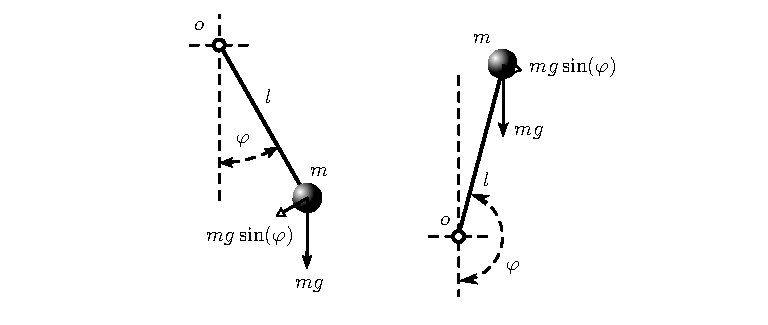
\includegraphics{Obr_Kyvadlo.pdf}
	}
	\vspace{-9mm}

	\figcaption{Kyvadlo}
	\label{Kyvadlo}
    }

	% \vspace{-3mm}
\end{center}

Pohybová rovnica opisujúca dynamiku rotačného pohybu kyvadla je v tvare
\begin{subequations} \label{PohRovKyvadla}
\begin{align}
		&ml^2 \ddot{\varphi}(t) + \beta \dot{\varphi}(t) + mgl\sin{\varphi(t)} = u(t) \label{PohRovKyvadlab} \\
		&ml^2 \ddot{\varphi}(t) = -\beta \dot{\varphi}(t) - mgl\sin{\varphi(t)} + u(t)
\end{align}
\end{subequations}
kde $u(t)$ [kg~m$^2$~s$^{-2}$] je externý moment sily pôsobiaci na rameno kyvadla, $\dot{\varphi}(t)$ [rad~s$^{-1}$] je uhlová rýchlosť a~$\ddot{\varphi}(t)$~[rad~s$^{-2}$] je uhlové zrýchlenie ramena kyvadla. Číselné hodnoty parametrov kyvadla sú uvedené v tabuľke~\ref{Parametre kyvadla}.

\begin{center}

\vbox{

\tabcaption{Parametre kyvadla}
\label{Parametre kyvadla}

\vspace{-3mm}

\begin{tabular*}{\textwidth}{ c @{\extracolsep{\fill}} c c}
    
    \toprule
    Parameter   & Hodnota    & Jednotky              \\
    \midrule
    $m$       & $1$   & kg             \\
    $l$    &  $1$  & m \\
    $g$   & $9,81$  & m s$^{-2}$ \\
    $\beta$  &  $2 \cdot 0,5 \cdot \sqrt{g/l}$ &  kg~m$^2$~s$^{-1}$ \\
    \bottomrule\

\end{tabular*}
} 

\vspace{-3mm}

\end{center}








\begin{itemize}[leftmargin=0pt, labelsep=3mm, itemsep=0pt]
    \item Vytvorte numerickú („počítačovú“) simuláciu časového priebehu výchylky kyvadla (kyvadlo ako nelineárny dynamický systém).
    \newline
    Alternatívy:
    \vspace{-6pt}
    \begin{itemize}[leftmargin=0pt, labelsep=4mm, itemsep=0pt]
        \item Schematické znázornenie pre implementáciu v prostredí MATLAB-Simulink.
        \item Implementácia s využitím všeobecného ODE solvera (bez Simulinku).
    \end{itemize}
\end{itemize}







\subsubsection{Kyvadlo -- simulácia rôznych scenárov}


\begin{itemize}[leftmargin=0pt, labelsep=3mm, itemsep=0pt]
    \item Simulujte priebeh výchylky kyvadla.
    \newline
    Scenáre:
    \vspace{-6pt}
    \begin{itemize}[leftmargin=0pt, labelsep=4mm, itemsep=0pt]
                \item[a)] Začiatočný stav: $\varphi = 0,25$ [rad], $\dot\varphi = 0$ [rad/s]. Vstupný signál $u(t) = 0$ [kg~m$^2$~s$^{-2}$].
                \item[b)] Začiatočný stav: $\varphi = 0,1$ [rad], $\dot\varphi = 1$ [rad/s].Vstupný signál $u(t) = 0$ [kg~m$^2$~s$^{-2}$].
                \item[c)] Začiatočný stav: $\varphi = 0$ [rad], $\dot\varphi = 0$ [rad/s]. Vstupný signál $u(t) = 3$ [kg~m$^2$~s$^{-2}$].
                \item[d)] Začiatočný stav: $\varphi = 0$ [rad], $\dot\varphi = 0$ [rad/s]. Vstupný signál $u(t) = 9,81$ [kg~m$^2$~s$^{-2}$].
                \item[e)] Začiatočný stav: $\varphi = 0$ [rad], $\dot\varphi = 0$ [rad/s]. Vstupný signál $u(t) = 9,82$ [kg~m$^2$~s$^{-2}$].
            \end{itemize}
\end{itemize}














\section{Poznámky k úlohám}


\paragraph{Schematické znázornenie dif. rovnice}

Pre schematické znázornenie dif. rovnice \eqref{eq:DR2R} je výhodné túto rovnicu prepísať tak, aby na ľavej strane bola len najvyššia derivácia neznámej, teda signál $\ddot y(t)$. Teda
\begin{equation} \label{eq:DR2Rs}
    \ddot y(t) = - a_1 \dot y(t) - a_0 y(t) + b_0 u(t)
\end{equation}
Na začiatku máme k dispozícii signál $\ddot y(t)$, teda
\begin{center}

    \vbox{%
    \makebox[\textwidth][c]{%
    \input{../fig_standalone/schB_pr2_k1.pdf_tex}
    }

    \vspace{-30mm}

    \figcaption{Bloková schéma rovnice \eqref{eq:DR2R}, krok prvý.}
    \label{schB_pr2_k1.pdf}
    }

\end{center}
Signál $\ddot y(t)$ je v podstate súčtom troch iných signálov.
\begin{center}

    \vbox{%
    \makebox[\textwidth][c]{%
    \input{../fig_standalone/schB_pr2_k2.pdf_tex}
    }

    \vspace{-5mm}

    \figcaption{Bloková schéma rovnice \eqref{eq:DR2R}, krok druhý.}
    \label{schB_pr2_k2.pdf}
    }

\end{center}
Prvý signál získame zosilnením signálu $\dot y(t)$ zosilňovačom so zosilnením $a_1$. Signál $\dot y(t)$ je možné získať integrovaním signálu $\ddot y(t)$.
\begin{center}

    \vbox{%
    \makebox[\textwidth][c]{%
    \input{../fig_standalone/schB_pr2_k3.pdf_tex}
    }

    \vspace{-5mm}

    \figcaption{Bloková schéma rovnice \eqref{eq:DR2R}, krok tretí.}
    \label{schB_pr2_k3.pdf}
    }

\end{center}
Druhý signál získame zosilnením signálu $y(t)$ zosilňovačom so zosilnením $a_0$. Signál $y(t)$ je možné získať integrovaním signálu $\dot y(t)$.
\begin{center}

    \vbox{%
    \makebox[\textwidth][c]{%
    \input{../fig_standalone/schB_pr2_k4.pdf_tex}
    }

    \figcaption{Bloková schéma rovnice \eqref{eq:DR2R}, krok štvrtý.}
    \label{schB_pr2_k4.pdf}
    }

\end{center}
Tretí signál získame zosilnením známeho (dostupného) signálu $u(t)$ zosilňovačom so zosilnením $b_0$. 
\begin{center}

    \vbox{%
    \makebox[\textwidth][c]{%
    \input{../fig_standalone/schB_pr2_kf.pdf_tex}
    }

    \figcaption{Bloková schéma rovnice \eqref{eq:DR2R}.}
    \label{schB_pr2_kf.pdf}
    }

\end{center}
Príslušné integrátori vo výslednej schéme musia mať začiatočné podmienky $y(0) = y_0$ a $\dot y(0) = z_0$ (podľa \eqref{eq:DR2R}).



\paragraph{Rozklad na sústavu dif. rovníc prvého rádu}

\noindent
Vo všeobecnosti platí, že každú diferenciálnu rovnicu vyššieho rádu je možné rozložiť (prepísať, transformovať) na sústavu rovníc prvého rádu. Ich počet je minimálne $n$, kde $n$ je rád pôvodnej dif. rovnice. Pre rovnicu \eqref{eq:DR2R} je rád rovnice 2, teda sústava bude mať minimálne 2 rovnice. 

Pre tieto dve nové rovnice je potrebné uvažovať dve veličiny, ktoré budú na mieste neznámej v nových diferenciálnych rovniciach. Označme ich $x_1(t)$ a $x_2(t)$.

Ako prvé zvoľme
\begin{equation} \label{volba1}
    x_1(t) = y(t)
\end{equation}
To znamená
\begin{equation}
    \dot x_1(t) = \dot y(t)
\end{equation}
čo však nie je v tvare aký hľadáme. Na pravej strane vystupuje pôvodná veličina $y(t)$.

Druhou voľbou preto nech je
\begin{equation} \label{volba2}
    x_2(t) = \dot y(t)
\end{equation}
pretože potom môžeme písať prvú diferenciálnu rovnicu v tvare
\begin{equation}
    \dot x_1(t) = x_2(t)
\end{equation}
Ostáva zostaviť druhú diferenciálnu rovnicu. 

Keďže sme zvolili \eqref{volba2}, tak je zrejmé, že platí
\begin{equation} 
    \dot x_2(t) = \ddot y(t)
\end{equation}
Otázkou je $\ddot y(t) = \ ?$ Odpoveďou je pôvodná diferenciálna rovnica druhého rádu. Upravme \eqref{eq:DR2R} na tvar
\begin{align}
    \ddot y(t) + a_1 \dot y(t) + a_0 y(t) &= b_0 u(t) \\
    \ddot y(t) &= - a_1 \dot y(t) - a_0 y(t) +  b_0 u(t) 
\end{align}
To znamená, že
\begin{equation}  \label{druhadr_1}
    \dot x_2(t) = - a_1 \dot y(t) - a_0 y(t) +  b_0 u(t) 
\end{equation}
čo však stále nie je požadovaný tvar druhej hľadanej diferenciálnej rovnice. Na pravej strane rovnice \eqref{druhadr_1} môžu figurovať len nové veličiny $x_1(t)$ a $x_2(t)$, nie pôvodná veličina $y(t)$. Stačí si však všimnúť skôr zvolené \eqref{volba1} a \eqref{volba2}. Potom môžeme písať
\begin{equation}  \label{druhadr_2}
    \dot x_2(t) = - a_1  x_2(t) - a_0 x_1(t) +  b_0 u(t) 
\end{equation}
čo je druhá hľadaná diferenciálna rovnica prvého rádu.

Diferenciálnu rovnicu druhého rádu \eqref{eq:DR2R} sme transformovali na sústavu diferenciálnych rovníc prvého rádu
\begin{align}
    \dot x_1(t) &= x_2(t) \\
    \dot x_2(t) &= - a_1  x_2(t) - a_0 x_1(t) +  b_0 u(t) 
\end{align}


\paragraph{Dif. rovnice jednosmerného motora}

V zmysle fyzikálnej podstaty jednosmerného s cudzím konštantným budením sú dif. rovnice opisujúce elektromagnetický a mechanický podsystém motora v~tvare \eqref{dfsv2}~a~\eqref{drms2}. Z hľadiska zostavenia numerickej simulácie je výhodné tieto rovnice upraviť do tvaru, ktorý zvýrazňuje jednotlivé signály v zmysle či ide o vstup alebo výstup a tým celkovú štruktúru dynamického systému. 

Navyše, je možné konštatovať (tu bez uvádzania podrobností), že ODE solver vo všeobecnosti (teda nástroj realizujúci numerickú simuláciu) pracuje s funkciou, ktorá realizuje funkčný vzťah medzi časovými deriváciami veličín a ich (nederivovanými) hodnotami. Preto je vhodné mať diferenciálne rovnice (prvého rádu) v tvare, keď na ľavej strane sú len samotné časové derivácie.

Rovnice \eqref{dfsv2} a \eqref{drms2} je možné písať v tvare
\begin{align}
    \frac{\text{d}i(t)}{\text{d}t} &= -\frac{R}{L} i(t) -\frac{C_{u\omega}}{L} \omega(t) + \frac{1}{L} u(t) \\
    \frac{\text{d}\omega(t)}{\text{d}t} &= \frac{C_{uM}}{J_m} i(t)
\end{align}

Ak by sme chceli ešte viac zvýrazniť vzťah medzi rýchlosťou zmeny signálov (časovou deriváciou), ich samotnými okamžitými hodnotami a inými signálmi, mohli by sme využiť maticový zápis, v tomto prípade:
\begin{align}
    \begin{bmatrix}
        \dot i(t) \\ \dot \omega(t)
    \end{bmatrix}
    =
    \begin{bmatrix}
        -\frac{R}{L} & -\frac{C_{u\omega}}{L} \\
        \frac{C_{uM}}{J_m} & 0
    \end{bmatrix}
    \begin{bmatrix}
        i(t) \\ \omega(t)
    \end{bmatrix}
    +
    \begin{bmatrix}
        \frac{1}{L} \\ 0
    \end{bmatrix}
    u(t)
\end{align}


\paragraph{Vzorová simulácia jednosmerného motora}

Vzorový výsledok simulácie štartu motora (mechanicky nezaťaženého) pri konštantnom napájacom napätí \lstyle{520}~[V] je na nasledujúcom obrázku:

\begin{center}

    \vbox{

    \makebox[\textwidth][c]{%
    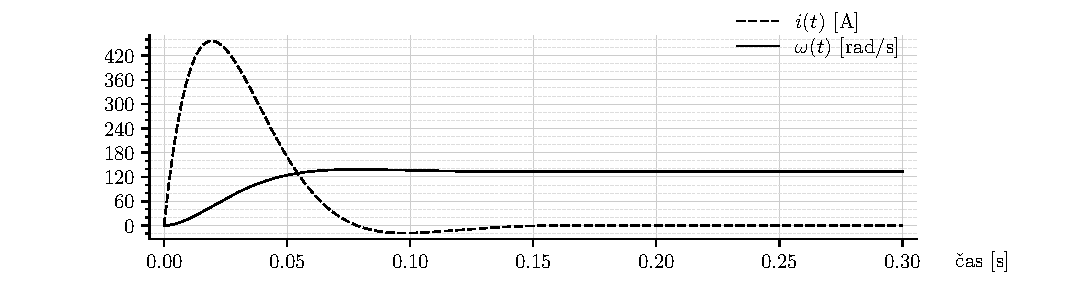
\includegraphics{kMRS03_fig_1.pdf}
    }

    \figcaption{Grafické znázornenie výsledku numerickej simulácie.}
    \label{Grafické znázornenie výsledku numerickej simulácie}

    }

\end{center}






\paragraph{Numerická simulácia kyvadla}

Diferenciálnu rovnicu opisujúcu kyvadlo \eqref{PohRovKyvadla} je možné prepísať na sústavu rovníc prvého rádu v tvare
\begin{align} \label{rovniceKyvSSpredpis}
    \begin{bmatrix} \dot x_1(t) \\ \dot x_2(t)  \end{bmatrix} = \begin{bmatrix} x_2(t) \\ -\frac{\beta}{ml^2} x_2(t) - \frac{g}{l} \sin\left( x_1(t) \right)  \end{bmatrix} + \begin{bmatrix} 0 \\ \frac{1}{ml^2} \end{bmatrix} u(t)
\end{align}
kde stavom kyvadla sú dve veličiny: uhol natočenia ramena kyvadla $\varphi$ a~uhlová rýchlosť ramena kyvadla $\dot\varphi$. Stavový vektor má preto dva prvky $x^{\mathsf{T}} = \begin{bmatrix} x_1 & x_2	\end{bmatrix}$, kde $x_1 = \varphi$ a~$x_2 = \dot\varphi$.

Vytvorme funkciu, ktorá realizuje sústavu diferenciálnych rovníc \eqref{rovniceKyvSSpredpis}, avšak, uvažujme, že vstupný signál $u(t)$ je nulový. Teda neuvažujme vstupný signál vôbec. Ešte inými slovami, externý moment sily je nulový, $u(t) = 0$ a preto potom možno písať
\begin{align} \label{fajnVektRov0}
	\begin{bmatrix}
		\dot{x}_1 \\ \dot{x}_2
	\end{bmatrix}
	&=
	\begin{bmatrix}
		x_2 \\ - \frac{\beta}{ml^2} x_2 - \frac{g}{l} \sin(x_1)
	\end{bmatrix}
\end{align}
Toto je autonómny nelineárny časovo-invariantný systém druhého rádu. Jeho správanie závisí len od začiatočného stavu na začiatku uvažovaného času.

Funkcia, ktorá realizuje uvedenú sústavu, môže byť nasledovná:
\lstset{style=mystyle}
\begin{lstlisting}[language=Matlab, title=Celý súbor PravaStr.m]
function dotx = PravaStr(t,x)

global m l g beta

dotx1 =  x(2);
dotx2 = - (beta/m*l^2)*x(2)  -  (g/l)*sin(x(1));

dotx = [dotx1; dotx2];

end
\end{lstlisting}

Vytvorme „hlavný skript“, v ktorom všetko potrebné nastavíme, a v ktorom budeme volať ODE solver. Ako prvé nech sú globálne premenné (v tomto prípade parametre kyvadla):

\vbox{%
\begin{lstlisting}[language=Matlab, title=Časť súbora hlSkript.m, name=hlSkript]
global m l g beta

m = 1; %kg
l = 1; %m
g = 9.81; %m/s^2
beta = 2*0.5*sqrt(g/l); %kgm^2/s
\end{lstlisting}
}

\noindent
Definujme časový vektor, ktorý určí pre aké časové okamihy ODE solver vráti numerické riešenie:
\begin{lstlisting}[language=Matlab, title=Časť súbora hlSkript.m, name=hlSkript]
timeVect = 0:0.1:5;
\end{lstlisting}
Zavolajme ODE solver, pričom ostáva zvoliť začiatočné podmienky - začiatočný stav kyvadla. Nech začiatočný stav je $x_1(0) = 0.25$ [rad] a~$x_2(0) = 0$ [rad/s].
\begin{lstlisting}[language=Matlab, title=Časť súbora hlSkript.m, name=hlSkript]
[t,x] = ode45(@(t,x) PravaStr(t,x), timeVect, [0.25; 0]);
\end{lstlisting}
Premenná \verb|x| teraz obsahuje dva stĺpce - prvý stĺpec je prvá stavová veličina a druhý stĺpec je druhá stavová veličina.
Pre nakreslenie vypočítaného riešenia:
\begin{lstlisting}[language=Matlab, title=Časť súbora hlSkript.m, name=hlSkript]
figure(1)
plot(t,x)
\end{lstlisting}
Výsledné numerické riešenie je graficky znázornené na obr.~\ref{cv3obr1}.

\begin{center}

    \vbox{

    \makebox[\textwidth][c]{%
    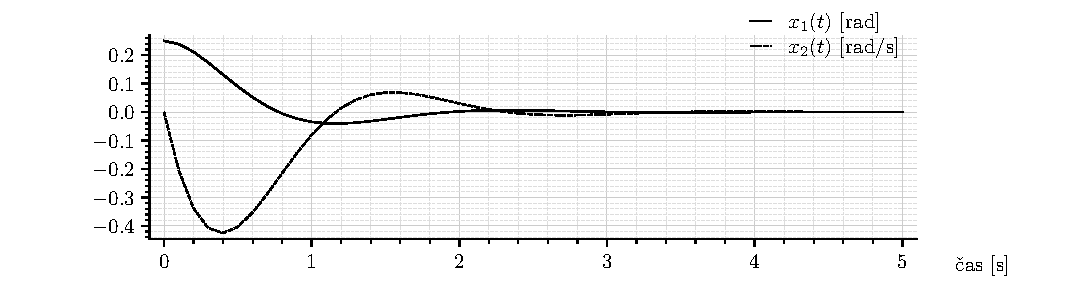
\includegraphics{cv03_fig_1.pdf}
    }

    \vspace{-4mm}

    \figcaption{Grafické zobrazenie numerického riešenia.}
    \label{cv3obr1}

    }

\end{center}

Na obr.~\ref{cv3obr1} ide však len o akési základné zobrazenie. Zmysluplnejšie by napríklad mohlo byť, ak by sme do grafu nakreslili len priebeh polohy (výchylky) kyvadla samostatne a navyše nie v radiánoch ale v stupňoch -- viď obr.~\ref{cv3obr2}. Pre takýto obrázok možno do hl. skriptu pridať:
\begin{lstlisting}[language=Matlab, title=Časť súbora hlSkript.m, name=hlSkript]
    figure(2)
    plot(t,x(:,1)*180/pi)
\end{lstlisting}

\begin{center}

    \vbox{

    \makebox[\textwidth][c]{%
    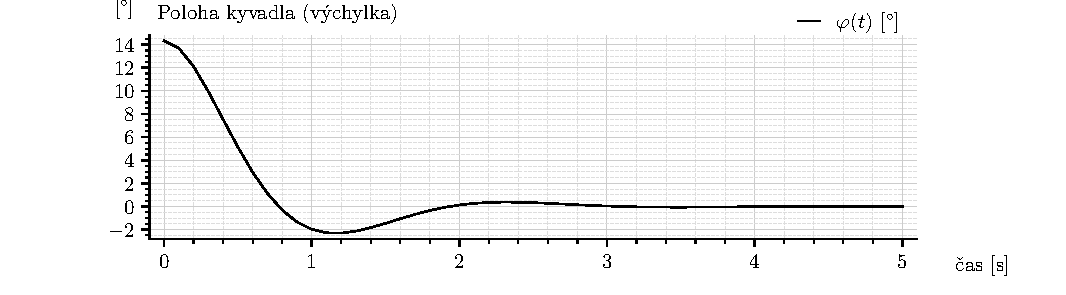
\includegraphics{cv03_fig_2.pdf}
    }

    \vspace{-4mm}

    \figcaption{Grafické zobrazenie priebehu polohy kyvadla.}
    \label{cv3obr2}

    }

\end{center}

Nech začiatočné podmienky (začiatočný stav) sú: $x_1(0) = 0.1$ [rad] a~$x_2(0) = 1$ [rad/s]. Pritom nech vstup $u(t)$ je stále nulový. Výsledok simulácie je na obrázku~\ref{cv3obr3}.

\begin{center}

    \vbox{

    \makebox[\textwidth][c]{%
    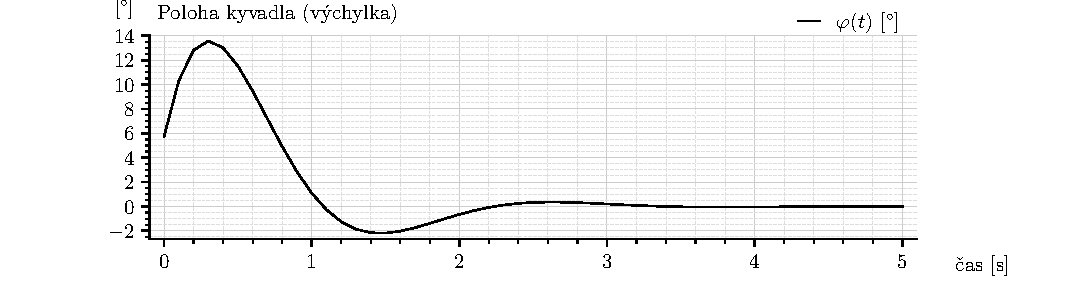
\includegraphics{cv03_fig_3.pdf}
    }

    \vspace{-4mm}

    \figcaption{Grafické zobrazenie priebehu polohy kyvadla.}
    \label{cv3obr3}

    }

\end{center}


Modifikujme pôvodnú funkciu a skrip v MATLAB-e tak, aby bolo možné simulovať nenulový vstupný signál $u(t)$.

Funkciu, ktorá realizuje sústavu diferenciálnych rovníc \eqref{rovniceKyvSSpredpis} aj so vstupným signálom $u(t)$:

\vbox{%
\begin{lstlisting}[language=Matlab, title=Celý súbor PravaStr\_u.m]
function dotx = PravaStr_u(t,x, u)

global m l g beta

dotx1 =  x(2);
dotx2 = - (beta/m*l^2)*x(2) - (g/l)*sin(x(1)) + (1/m*l^2) * u;

dotx = [dotx1; dotx2];

end
\end{lstlisting}
}

Vytvorme „hlavný skript“, v ktorom všetko potrebné nastavíme, a v ktorom budeme volať ODE solver:

\vbox{%
\begin{lstlisting}[language=Matlab, title=Súbor hlSkript\_u.m]
global m l g beta

m = 1; %kg
l = 1; %m
g = 9.81; %m/s^2
beta = 2*0.5*sqrt(g/l); %kgm^2/s

u = 3

[t,x] = ode45(@(t,x) PravaStr_u(t,x,u), [0 10], [0; 0]);

figure(3)
plot(t,x(:,1)*180/pi)
\end{lstlisting}
}

\noindent
Simulujme prípad keď napríklad $u(t) = 3$ [kg m$^2$ s$^{-2}$] (pozn.: pre lepšiu názornosť uvažujme začiatočné podmienky nulové). Výsledok simulácie je na obrázku~\ref{cv3obr4}.

\begin{center}

    \vbox{

    \makebox[\textwidth][c]{%
    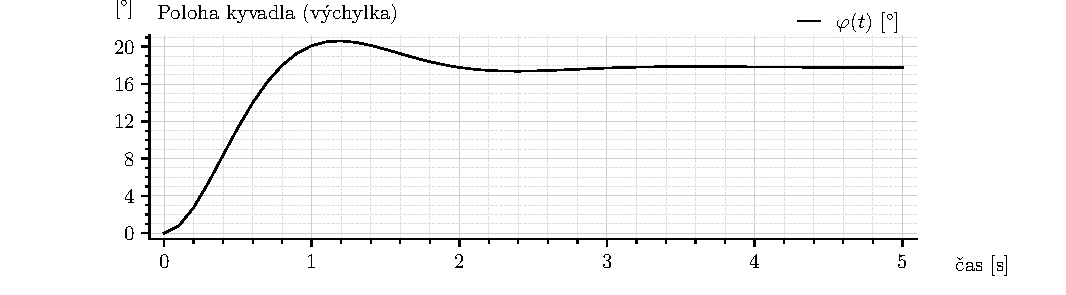
\includegraphics{cv03_fig_4.pdf}
    }

    \vspace{-4mm}

    \figcaption{Grafické zobrazenie priebehu polohy kyvadla.}
    \label{cv3obr4}

    }

\end{center}

Zaujímavý prípad je, keď $u(t) = 9,81$ [kg m$^2$ s$^{-2}$]. Výsledok simulácie je na obrázku~\ref{cv3obr5}.

\begin{center}

    \vbox{

    \makebox[\textwidth][c]{%
    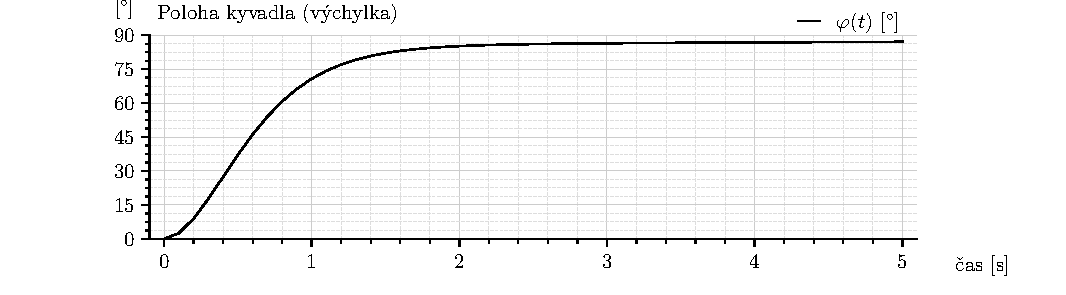
\includegraphics{cv03_fig_5.pdf}
    }

    \vspace{-4mm}

    \figcaption{Grafické zobrazenie priebehu polohy kyvadla.}
    \label{cv3obr5}

    }

\end{center}

\noindent
Avšak, lepšie sa to ukáže, ak predĺžime časový vektor (čas simulácie) -- viď obrázok~\ref{cv3obr6}. Je zrejmé, že kyvadlo sa približuje k hodnote 90 stupňov.

\begin{center}

    \vbox{

    \makebox[\textwidth][c]{%
    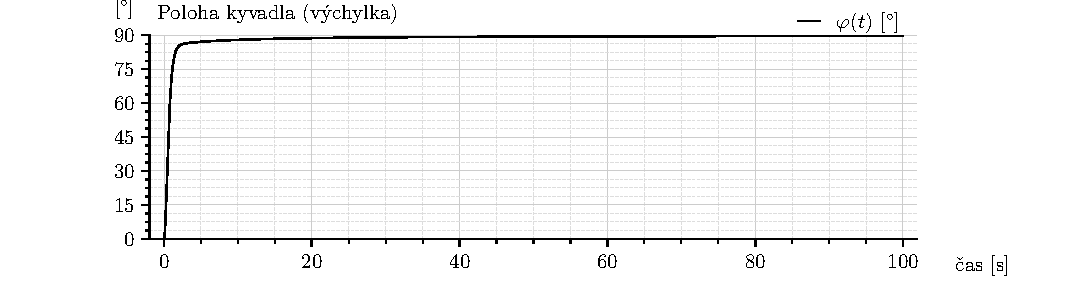
\includegraphics{cv03_fig_6.pdf}
    }

    \vspace{-4mm}

    \figcaption{Grafické zobrazenie priebehu polohy kyvadla.}
    \label{cv3obr6}

    }

\end{center}

\noindent
Čo sa stane ak $u = 9,82$ [kg m$^2$ s$^{-2}$]? (obr.~\ref{cv3obr7})

\begin{center}

    \vbox{

    \makebox[\textwidth][c]{%
    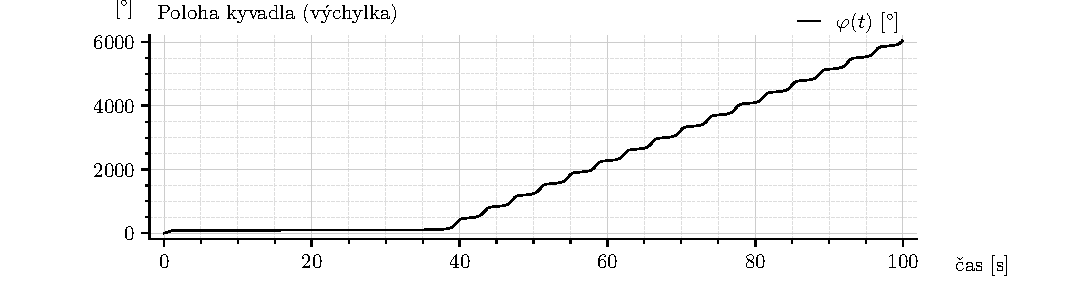
\includegraphics{cv03_fig_7.pdf}
    }

    \vspace{-4mm}

    \figcaption{Grafické zobrazenie priebehu polohy kyvadla.}
    \label{cv3obr7}

    }

\end{center}

















\end{document}
